\documentclass{article}

\usepackage[english]{babel}
\usepackage{authblk}
\usepackage[a4paper,top=2cm,bottom=2cm,left=3cm,right=3cm,marginparwidth=1.75cm]{geometry}
\usepackage{amsmath}
\usepackage{graphicx}
\usepackage[colorlinks=true, allcolors=blue]{hyperref}
\usepackage{gensymb}
\usepackage{textcomp}
\usepackage[backend=biber, style=nature]{biblatex}
\usepackage{csquotes}

\addbibresource{references.bib}

\title{Predicting Ensemble Width and Location in Binaural Recordings of Music with Convolutional Neural Networks}
\author[1,*]{Paweł Antoniuk}
\author[1]{Sławomir Zieliński}
\affil[1]{Faculty of Computer Science, Białystok University of Technology}
\affil[*]{Corresponding author: pawel.antoniuk@sd.pb.edu.pl}
\date{}

\begin{document}
\maketitle

\begin{abstract}
  Binaural audio technology has been around for many years, but its popularity has dramatically increased over the past decade due to advancements in virtual reality and streaming technologies. Along with its growing popularity, the quantity of publicly accessible binaural audio materials has also expanded. Consequently, there is now a need for automated and objective measurements of spatial content information, with ensemble width and location being the most important. This study presents a novel method for predicting ensemble width and location in binaural recordings. To this end, 30 head-related transfer functions and 192 binaural music recordings from publicly accessible multi-track recording repositories were used to synthesize 23,040 binaural recordings. The synthesized recordings were then used to train a multi-task convolutional neural network prediction model, the aim of which was to predict the width and location of the ensemble for unseen recordings. The results indicate that models of ensemble breadth and position can be successfully constructed with low prediction errors --- $4.76\degree$ ($\pm0.10\degree$) for ensemble location and $8.57\degree$ ($\pm0.19\degree$) for ensemble width. This approach is the first of its kind to predict both ensemble width and location, offering a more accurate representation of spatial properties. This suggests significant potential for advancing spatial audio applications in virtual reality and streaming technologies, by providing audio engineers with tools that can leverage these methods to enhance spatial audio experiences.
\end{abstract}

\section{Introduction}

The human auditory system demonstrates exceptional proficiency in segregating, localizing, and interpreting diverse auditory signals, despite being limited to two ears. This capability arises from the intricate analysis of temporal, amplitude, and spectral disparities, a process termed binaural hearing \cite{blauert_spatial_1996}, which enables precise localization of sound sources in complex auditory environments. An important advantage of binaural hearing is demonstrated by the `cocktail party effect', which showcases the system's capacity to concentrate on individual sounds while suppressing background noise \cite{cherry_experiments_1953}. An understanding of the auditory system is essential for comprehending its limits and creating more immersive binaural experiences for entertainment purposes \cite{zhang_surround_2017}. It also helps to improve hearing aid devices by enhancing auditory signal reception and improving spatial awareness \cite{thiemann_speech_2016}.

The advancement of sophisticated machine learning techniques, particularly deep learning networks, has prompted an intriguing exploration of the extent to which these tools can emulate the human auditory system without relying on advanced spatial audio feature engineering, traditionally employed in audio source localization tasks \cite{yang_deepear_2022, vera-diaz_towards_2018, pang_multitask_2019}. To investigate this, the study developed an audio localization method based on a multi-task convolutional neural network (CNN) model.

Inspired by the fact, that humans tend to localize sound sources in groups rather than individually \cite{bregman_auditory_1990, rumsey_spatial_2002}, the objective of the proposed model is to predict ensemble location and width instead of positions of individual sources. This study is unique as it not only conceptualized the method but also tested it on a vast, real-life music corpus of 23,040 binaural excerpts that were synthesized using 192 multi-track music recordings and 30 publicly available head-related transfer functions (HRTFs) from various sources. The music recordings encompassed various genres, including rock, jazz, pop, and classical music.

The developed method has the potential to be highly beneficial in automated assessment tasks, where a significant number of binaural recordings must be evaluated and labeled in terms of their spatial content information. This may assist audio engineers in objectively assessing and segregating binaural audio recordings with regard to their spatial content. Furthermore, it could facilitate the development of an autonomous web-crawler bot that will collect binaural recordings from publicly accessible repositories and label them according to the spatial properties of the sound sources, such as the location of the music ensemble or the sparsity of audio source positions.

The findings demonstrate that this method is effective in accurately predicting the spatial characteristics of sound sources in near-real-world scenarios. Furthermore, this paper presents an experiment framework that allows for the objective measurement of a binaural localization technique in an objective manner, utilizing a large-scale dataset synthesized from real-world examples of music signals (for other use cases for this framework, see \cite{antoniuk2023blind, zielinski_automatic_2022, zielinski_spatial_2022, zielinski_comparison_2020}). One of the key advantages of the proposed method is that it does not assume the number of audio sources. However, a significant limitation of this study is the lack of reverberation in the synthesized recordings, which represents a material for future research.

The remainder of this paper is organized as follows. In Section \ref{sec:related-studies}, related studies are presented. The description of the method developed as part of this study is provided in Section \ref{sec:methodology}. This section also includes a detailed definition of ensemble width and the description of the experiments that was used to evaluate this method. Section \ref{sec:results} discusses the results of the method-evaluation experiments conducted in this study. Finally, the paper is summarized in Section \ref{sec:conclusions}.

\section{Related studies}
\label{sec:related-studies}

The majority of existing literature on the subject of sound source localization employs techniques that leverage the advantages of microphone arrays with more than two channels \cite{kaveh_statistical_1986, pavlidi_real-time_2012, pan_multi-tone_2021, hahmann_sound_2022, chung_sound_2022, liu_sound_2022}. In the context of sound source localization in binaural signals, the predominant focus of research is on the identification of individual sound sources, rather than groups of sounds \cite{dietz_auditory_2011, may_probabilistic_2011, may_binaural_2012, woodruff_binaural_2012, may_robust_2015, ma16c_interspeech, ma_exploiting_2017, benaroya_binaural_2018}. In terms of source direction of arrival (DOA) methods, the majority of research assumes a fixed number of sound sources \cite{pang_multitask_2019, vecchiotti19, ma_exploiting_2017, woodruff_binaural_2012, s_spatiogram_2021}, which limits its practical applications as this information is rarely known in real-life binaural recordings. Moreover, the majority of studies have focused on relatively homogeneous signals, namely speech \cite{dietz_auditory_2011, may_probabilistic_2011, may_binaural_2012, woodruff_binaural_2012, may_robust_2015, ma16c_interspeech, ma_exploiting_2017, benaroya_binaural_2018, wang_binaural_2020, liu_multiple_2018, yang_deepear_2022, ma_robust_2018}.

In contrast to the aforementioned studies, the proposed method is not limited by the number of sources. Furthermore, the approach is not limited to speech and has been applied to much more diverse musical datasets, including sound sources such as instruments and vocals. In contrast to previous studies that have focused on individual sources, the proposed method does not aim to separate them, but rather considers them as an ensemble, or in this case, a musical ensemble. This approach is inspired by the way real musical ensembles are arranged on stage. To the authors' knowledge, this is one of the first methods to localize ensemble width (see \cite{antoniuk2023blind} for the previous ensemble-width-related study), and the first to localize both ensemble position and width simultaneously using a multi-task model.

Sound localization methods can be classified into two primary categories based on the implementation of their underlying algorithms: glass-box and black-box. The glass-box methods, which are more traditional in the literature, rely on manual designing algorithms that mimic the auditory system to explicitly extract key features from the signal for location prediction, such as one of combination of the following: interaural level difference, interaural time difference, interaural coherence or interaural phase difference (see \cite{blauert_spatial_1996} for features description). In contrast, black-box methods typically employ only basic feature engineering and rely heavily on modern machine learning techniques to both extract features and make the final prediction. Consequently, they are less reliant on manual intervention (see \cite{vecchiotti19} for an example). The black-box algorithm extracts features implicitly and internally, without knowledge of their internal purpose or the equivalent of the human auditory system. This renders such methods less transparent and less predictable. This, in conjunction with the fact that they are typically implemented with deep neural networks with a large number of learning parameters, necessitates the development of them with the use of very large datasets, typically comprising hundreds of thousands of examples.

\section{Methodology}
\label{sec:methodology}

Experiments in this study were conducted on 23040 binaural recordings of music. The binaural recordings were synthesized semi-automatically using 192 multi-track publicly-available music recordings and 30 HRTF databases. For each multi-track recording and HRTF database pair, four binaural recordings were synthesized for different random ensemble parameters --- its location $\theta$ and width $\theta$ --- as defined in Section \ref{subsec:ensemble-definition}. Both parameters were drawn from uniform random distribution.

\subsection{Ensemble location and width definition}
\label{subsec:ensemble-definition}

The primary objective of the model developed in this study is to predict the ensemble location ($\theta$) and width ($\omega$), as illustrated in Figure \ref{fig:scene}. The ensemble is defined as a group of audio point sources. The ensemble width $\omega$ is defined as the angular width between two extreme point sources, while the ensemble location $\theta$ represents the middle angle between two extreme sound sources.

\begin{figure}[ht]
  \centering
  \includegraphics[width=\linewidth]{../pictures/scene.png}
  \caption{\label{fig:scene}Illustration of ensemble width ($\omega$) and ensemble location ($\theta$) relative to the direction of the head. Black dots represent the positions of audio sources. The ensemble location ($\theta$) is defined as the angular position of the center of the ensemble relative to the direction the head is turned. The ensemble width ($\omega$) is defined as angular distance between two extreme audio sources. }
\end{figure}

\subsection{Synthesis of binaural music recordings}

\subsection{Spectrogram conversions of binaural music recordings}

\begin{figure}
  \centering
  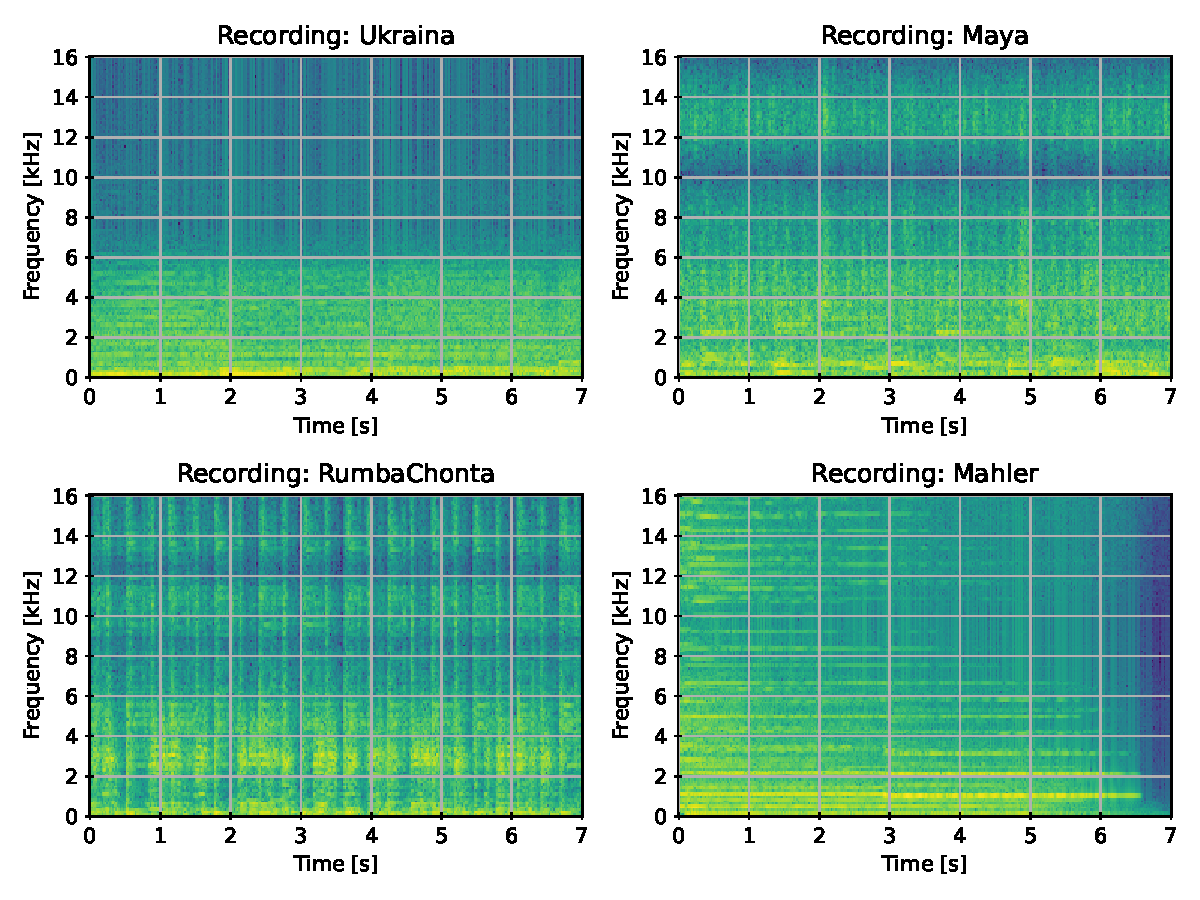
\includegraphics[width=\linewidth]{../figures/samples.pdf}
  \caption{\label{fig:samples}An illustrative example of the magnitude spectrograms generated from synthesized binaural recordings of music. Each spectrogram was derived from a different randomly selected binaural music recording. These spectrograms were subsequently employed as input data for training and assessing the convolutional neural network (CNN) in this study. }
\end{figure}

Prior to being fed into the model, the binaural recordings of music were transformed into magnitude spectrograms. Figure \ref{fig:samples} illustrates example spectrograms for four distinct binaural recordings of music. It should be noted that the original spectrograms were stored in a floating-point-precision matrix format.

\subsection{Convolutional neural network topology}
\subsection{Model training and evaluation}

\section{Results}
\label{sec:results}

\begin{figure}[ht]
  \centering
  \begin{minipage}[t]{0.45\linewidth}
    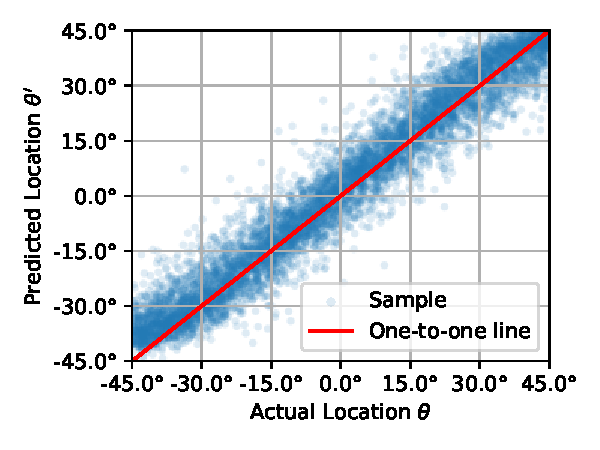
\includegraphics[width=\linewidth]{../figures/actual_vs_predicted_location.pdf}
    \caption{\label{fig:actual_vs_predicted_location}A comparison between the actual ensemble location $\theta$ and the predicted ensemble location $\theta'$ for a single iteration (of the total five) }
  \end{minipage}
  \hspace{0.5cm}
  \begin{minipage}[t]{0.45\linewidth}
    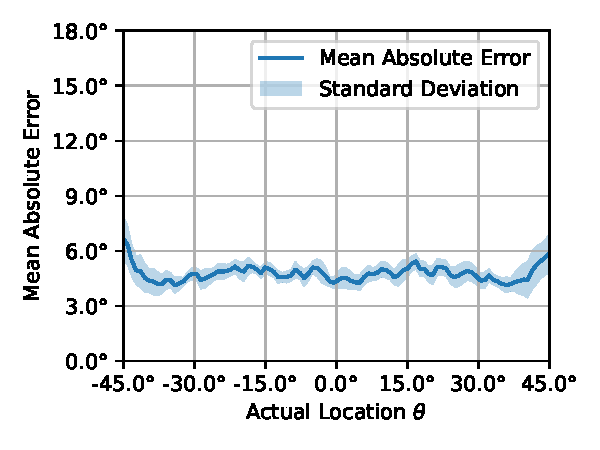
\includegraphics[width=\linewidth]{../figures/mae_location.pdf}
    \caption{\label{fig:mae_location}The impact of the actual ensemble width $\omega$ on the mean absolute prediction error, averaged across all five iterations, with indicated standard deviation.}
  \end{minipage}
\end{figure}

Figure \ref{fig:actual_vs_predicted_width} illustrates the comparison between the actual and the predicted ensemble width. The results demonstrate that the model exhibits better prediction quality for narrower ensemble widths ($12.44\degree$ for $\omega>80\degree$) and that its performance deteriorates with the increase of the ensemble width ($Z\degree$ for $W\degree$). Figure \ref{fig:mae_width} further demonstrates that the relationship between the prediction error and the actual width is not linear, exhibiting a depression between 60 and 75 degrees. This suggests, that the ensemble width has a significant impact on the ensemble width estimation.

\begin{figure}[ht]
  \centering
  \begin{minipage}[t]{0.45\linewidth}
    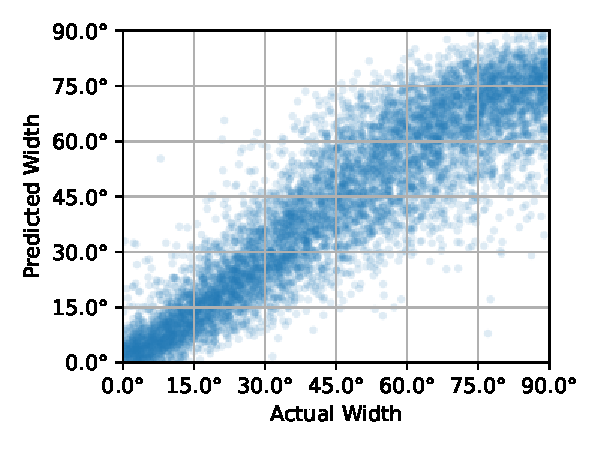
\includegraphics[width=\linewidth]{../figures/actual_vs_predicted_width.pdf}
    \caption{\label{fig:actual_vs_predicted_width}A comparison between the actual ensemble width $\omega$ and the predicted ensemble width $\omega'$ for a single iteration (of the total five) }
  \end{minipage}
  \hspace{0.5cm}
  \begin{minipage}[t]{0.45\linewidth}
    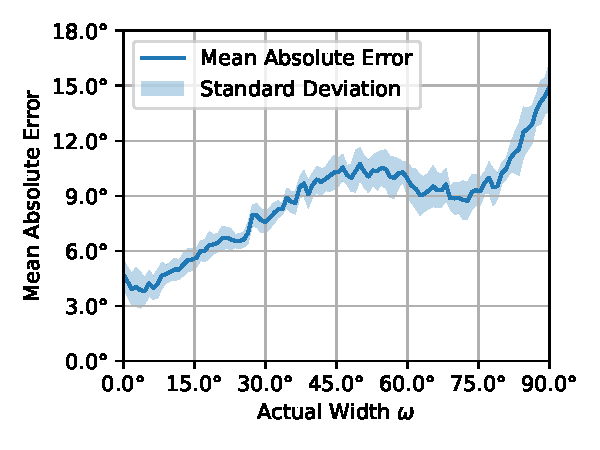
\includegraphics[width=\linewidth]{../figures/mae_width.pdf}
    \caption{\label{fig:mae_width}The impact of the actual ensemble width $\omega$ on the mean absolute prediction error, averaged across all five iterations, with indicated standard deviation.}
  \end{minipage}
\end{figure}

In contrast to the correlation between ensemble width and its prediction error, there is no significant relationship between the actual location and its prediction error, as illustrated in Figures \ref{fig:actual_vs_predicted_location} and \ref{fig:mae_location}. This finding indicates that the model's capabilities for localizing the center of the ensemble is robust, unaffected by the actual spatial positioning of the ensemble, including lateral locations.

\begin{figure}[ht]
  \centering
  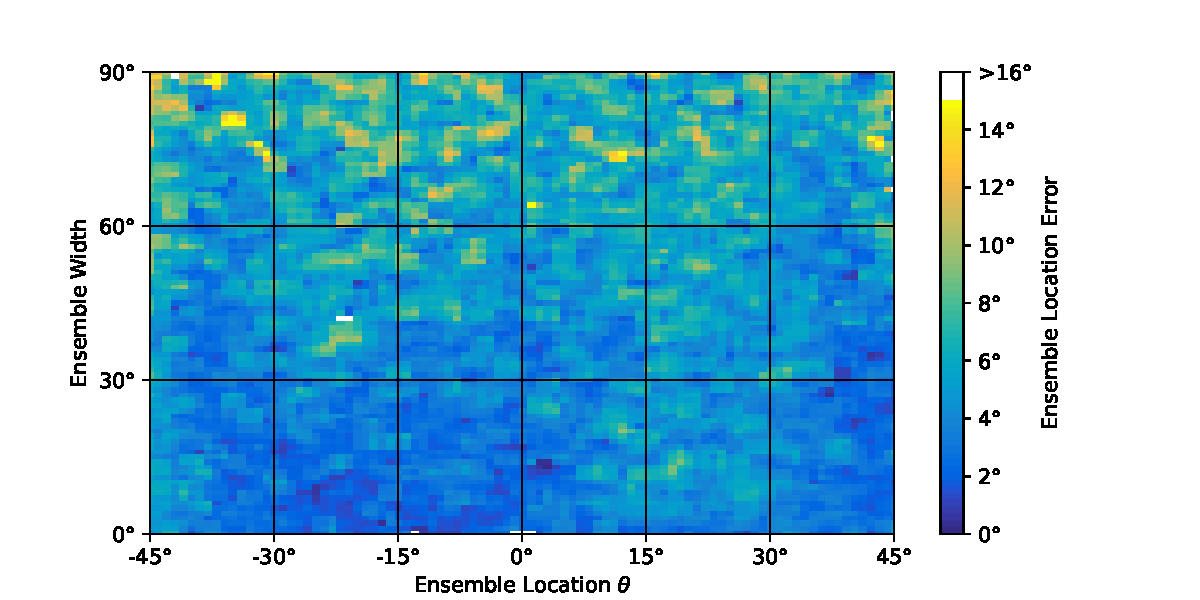
\includegraphics[width=\linewidth]{../figures/map_mae_location.pdf}
  \caption{\label{fig:map_mae_location}The heatmap that illustrates the mean absolute error (MAE) of ensemble location distribution across different ensemble locations (x-axis) and ensemble widths (y-axis). The color intensity corresponds to the MAE values, with lighter areas indicating higher errors.}
\end{figure}

\begin{figure}[!htb]
  \centering
  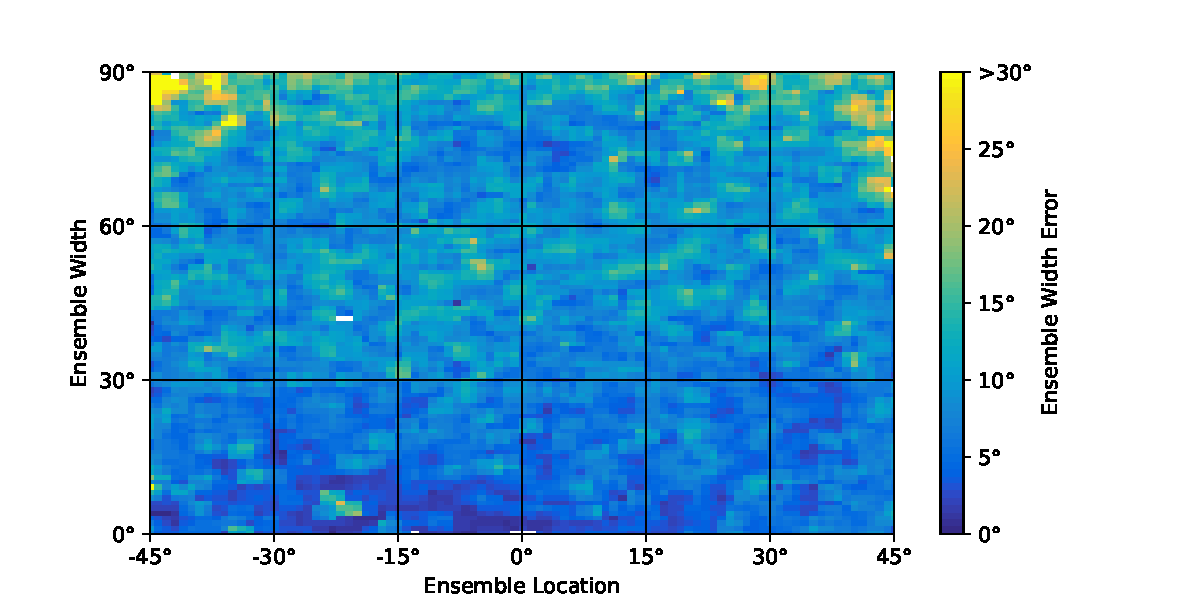
\includegraphics[width=\linewidth]{../figures/map_mae_width.pdf}
  \caption{\label{fig:map_mae_width}The heatmap that illustrates the mean absolute error (MAE) of ensemble width distribution across different ensemble locations (x-axis) and ensemble widths (y-axis). The color intensity corresponds to the MAE values, with lighter areas indicating higher errors. Notably, the values between $30\degree$ and $60\degree$ on the y-axis exhibit unexpectedly higher MAE values region --- please see Figure \ref{fig:mae_width} for comparison. }
\end{figure}

Figure \ref{fig:map_mae_location}  illustrates the influence of both ensemble width and location on mean absolute error for ensemble location. This figure provides a more detailed view of the data presented in Figure \ref{fig:mae_location}. The figure indicates a slight asymmetry. Similarly, Figure \ref{fig:map_mae_width} illustrates the influence of both ensemble width and location on mean absolute error for ensemble width.


\section{Conclusions}
\label{sec:conclusions}

\clearpage

\printbibliography

\end{document}
